\documentclass[10pt,letterpaper]{article}
\usepackage{amsmath}
\usepackage{amsfonts}
\usepackage{amssymb}
\usepackage[english]{babel}
\usepackage{breakurl}
\usepackage[superscript]{cite}
\usepackage{draftwatermark}
\usepackage{fancyhdr}
\usepackage{float}
\usepackage[margin=1in]{geometry}
\usepackage{graphicx}
\usepackage{hyperref}
\usepackage[utf8]{inputenc}
\usepackage{listings}
\usepackage{makeidx}
\usepackage{multicol}
\usepackage{nth}
% \usepackage[default,scale=1.0]{opensans} % CHANGED:
\usepackage{pgf-umlcd}
\usepackage{setspace}
\usepackage{siunitx}
\usepackage{svg}
\usepackage{subcaption}
\usepackage{tikz}
\usepackage{url}

% [PREAMBLE]
% Custom commands
\newcommand{\ts}{\textsubscript}
\newcommand{\bs}{\bigskip}

% !!! Global variables
\newcommand{\titletext}{Exploration of Design Patterns in Game Development}

% Change color of UML diagrams
\renewcommand{\umltextcolor}{black}
\renewcommand{\umldrawcolor}{black}
\renewcommand{\umlfillcolor}{white}

% Use differnet symbols for footnotes to avoid ambiguity with citations
\renewcommand{\thefootnote}{\roman{footnote}}

% New flags
\newif\iftwocolumns

% Set flags
% \twocolumnsfalse
\twocolumnstrue

% Double spacing
% \doublespacing

% Watermark
\SetWatermarkText{Draft}
\SetWatermarkScale{5}
\SetWatermarkColor[gray]{0.95}

% Use hyphans to break up urls
\def\UrlBreaks{\do\/\do-}

% Hyper ref setup
\hypersetup{
	colorlinks=true,
	citecolor=black,
	linkcolor=black,
	filecolor=black,
	% urlcolor=blue,
	urlcolor=black,
	pdftitle={APSC 310 Technical Report - Muchen He},
	bookmarks=true
}
\urlstyle{same}

% Page semantics
\pagestyle{fancy}

% Header
\fancyhead[L]{\MakeUppercase{APSC 310}}
\fancyhead[R]{Muchen He}
\fancyfoot{}
\fancyfoot[C]{\thepage}

% Page indent
\parindent 0ex

% Metadata
\author{Muchen He}
\title{APSC 310 Work Term Technical Report}

% Listings style
\lstdefinestyle{codestyle}{
	basicstyle=\footnotesize,
	frame=single,
	tabsize=4
}
\lstset{style=codestyle}

% [DOCUMENT]
\begin{document}

% [TITLE PAGE]
\begin{titlepage}
	\begin{center}
		\vspace*{2in}
		\line(1, 0){400}\\
		\Huge{\textbf{\titletext{}}}\\[0.2cm]
		\large{\textbf{Technical Work Term Report (Work Term 3)}}\\[1cm]
		\Large{\textbf{APSC 310}}\\[1cm]
		\includegraphics[width=1.4cm]{assets/ubc}\\
		\textbf{University of British Columbia}\\
		\line(1, 0){400}\\
		\vfill
		\Large{Muchen He}\\
		\large{Associate Developer, BioWare Edmonton}\\
		Student Number: 44638154\\

		\today \\
	\end{center}
\end{titlepage}

% [TOC]
\setcounter{secnumdepth}{3}
\tableofcontents
\thispagestyle{empty}
\clearpage

% [PREFACE]

% Set page numbering to roman for preface
\pagenumbering{roman}

% !!! Preface
\section*{Preface \& Foreword}
\addcontentsline{toc}{section}{Preface \& Foreword}

% Purpose
\subsection*{Purpose}
\addcontentsline{toc}{subsection}{Purpose}

The purpose of this report is to explore and observer different kinds of theoretical methods nad patterns and how they're used ot develop components that make up a game.\bs
\\
As well to consolidate my knowledge as a whole in the industry as design patterns are software development concepts and potentially applicable elsewhere in the tech industry.

% Background
\subsection*{Background}
\addcontentsline{toc}{subsection}{Background}

(Working at EA-Bioware)
(Associate Developer (Programmer) for game Anthem)
(Using modern game engine Frostbite)

% Scope
\subsection*{Scope of Coverage}
\addcontentsline{toc}{subsection}{Scope of Coverage}

(The scope of this report)(Covers many design patterns outlined in ``Gang of Four'')(Will not cover detailed breakdown, explanation, and specification of existing proprietary tech; i.e. extended code from the game or Frostbite engine)\bs
\\
The technical coverage cited in this report is limited because the co-op work term position is working in UI/UX. Thus I lack understanding in other areas of the game such as character handling, world rendering, etc. Many of the workflows I describe in this report may only apply to UI/UX development within this project.\bs
\\
As the scope of game development or software development extends wide in breadth, this report will not thoroughly cover topics of object oriented programming, development methodologies, specific syntax in a programming language, specific implementations of algorithms in a programming language, and psychology of UI/UX.

% (Other) Contributors
\subsection*{Contributors}
\addcontentsline{toc}{subsection}{Contributors}

(Gibson, Tim - senior software lead, manager: contribution by supervising the report and giving advice) 
(Johnson, Chris - supervisor, programmer, assisted in design pattern example)
(Steadman, Andrew)

\newpage

% !!! [SUMMARY]
\section*{Summary}
\addcontentsline{toc}{section}{Summary}
\newpage

% [List of Figures/Tables]
% \thispagestyle{empty}
\listoffigures
\addcontentsline{toc}{section}{List of Figures}
\listoftables
\addcontentsline{toc}{section}{List of Tables}
\newpage

% Reset page counter
\pagenumbering{arabic}
\setcounter{page}{1}
\setcounter{section}{0}

% !!! [INTRODUCTION]
\iftwocolumns
\begin{multicols}{2}
\fi

% ??? [DISCUSSION]
\section{Introduction}

This enters the discussion portion of the report. We will analyze the current processes in game development for UI/UX at BioWare. Then look at some of the more theoretical, template solutions known as design patterns in later sections and draw comparisons. We will also look into how the design patterns would be used in a general sense in game development (not specific to BioWare or Bioware's current project, Anthem).

\subsection{Game Development Overview}

% There are many parts to a video game. It can be grouped into: rendering, physics / simulation, AI, UI, sound / music. online, controls (input handling), online / networking. All tied together by the game engine.\\

% Having all the systems working together monolithically is bad, because it's difficult to maintain, prone to errors and bugs, and hard to collaborate as sub-systems are too tightly coupled.\\

% Talk about the video game industry -> video game development
% -> video game roles
A major portion of the video game market consists of AAA video games. These are titles with very high production value, large budget, and typically consists of a team of hundreds of developers. These developers consist of artists, scripters, programmers, managers, etc. Many of these roles are further grouped into sub-teams such as rendering, physics/simulation, AI, UI/UX, sound design, music production, networking, etc. Individual developers are specialized to work on one part of the game, with the exception of leads, managers, and other executives.

\subsubsection{Game Engine}
Developers will use a game engine so that many people can work on the project at once. The game engine is generally highly optimized for graphics rendering, physics simulation (such as collision detection), and object handling.\bs

The Frostbite engine is the game engine widely adopted at Electronic Arts (EA) studios. It was originally developed by Digital Illusions CE (DICE).\cite{frostbite}\cite{frostbite-wiki} As expected, the game engine is a piece of software, thus it is prone to software development problems that design patterns are ought to solve.

\subsection{Game Building}

Programmers make primitive entities such as an abstract UI widget, as well as the system that manages these entities.\bs
\\
The scripters and artists then use these entities in \textit{schematics} or \textit{blueprints}, which are used for visual scripting blocks of game content that contains logic and input/output together. Figure \ref{fig:unreal-blueprint} shows an example of what it looks like.\bs
\\
These schematics are in game levels, UI widgets, and prefabricated logic blocks (LogicPrefab). Thousands of these make up functionalities in a game, and are all handled by the game engine.

\begin{figure}[H]
	\centering
	\includegraphics[width=0.49\textwidth]{assets/unreal-blueprint}
	\caption{Blueprint (schematics) for development in Unreal Engine\cite{unity-vs-unreal}}
	\label{fig:unreal-blueprint}
\end{figure}

\subsubsection{Role of Programmers}

At BioWare, most game programmers work with code (in C++ and C\#). Programmers are specialized to develop in-game entities, or tools for scripters, designers, and artists. Programmers also integrate systems together, such as making mouse inputs interact with hitzones widgets, which interacts with graphical widgets or animation timelines.\footnote{Animation timelines are timeline that describe how a particular object will animate. Example: a fade in.}

\subsection{Object Oriented Programming}

\textit{Object oriented programming} (OOP) is a programming paradigm centered around interaction of encapsulated objects. Objects have its own functions (methods), input and output (\textit(getters) and \textit(setters)), state and memory (member variables). OOP emphasizes on encapsulation which makes software structure easier to organize and debug. OOP allows programmers to define well-defined boundaries between features or objects. OOP also enables \textit{polymorphism} and \textit{inheritance} which are important in abstraction and organization of code.\cite{oop}\bs
\\
Although we will not go into depth into the subject of object oriented programming, it is vital to understand that OOP is basis of most modern game development due to its benefits of reusability, refactoring, extensibility/scalability, maintenance, and efficiency\cite{oop}. Nearly all of the design patterns explored here are utilizing OOP concepts in some way. 

\subsection{Design Pattern}

TODO:
Design patterns are reusable, general, abstract solutions to common problems in software development.\cite{sm-designpatterns} Design patterns are meant to be used when there no problems actually exist -- doing so would cause excess undesired complexity.\cite{gof}\bs
\\
Throughout the exploration in this report, we will see that all the patterns loosely fit into three categories of benefits: performance optimization, readability/maintainability improvement, organization/structure/scalability improvement. We use these three categories to evaluate the usefulness of the design patterns in game development. (TODO:)

\subsubsection{Antipatterns}
Software written without care are difficult to maintain, prone to bugs and errors, and hard to collaborate. Software written with these ``hacks'' are known as \textit{antipatterns}, where there is more negative consequences than the benefits of its solution. Antipatterns are counter parts to correctly implemented design patterns.\cite{sm-antipatterns}\bs
\\
Avoid antipatterns as much as possible. Exploring the negative effects of antipatterns is not part of the scope of this report.

\subsubsection{Gang of Four}

In software development, the phrase ``Gang of Four'' refers to the four authors of the Design Patterns book, Erich Gamma, Richard Helm, Ralph Johnson, and John Vlissides\cite{gof-wiki}\cite{gof}. The book features the most common design patterns widely in use today.\bs
\\
The design patterns featured in the book outlines the classical design patterns. Thus, many patterns would not be applicable as more recent revisions of programming languages (Python, c++11, etc.). This is because design patterns are inherently solutions / workarounds to limitations of the programming language. As there are more improvement in the usability of the language, certain design patterns (such as the \textit{template} pattern) are implemented less as it's less complex, less error prone, and easier to use the existing features built-in to a language.


\section{Creational Design Patterns}

Creational design patterns involves with object creation.\cite{sm-creationaldp} This is especially useful in game development, such as when we need to create many trees or bushes in a level of a game. These patterns become more useful when the objects we're trying to create have relationships, such as \textit{inheritance}, to other objects.

\subsection{Builder}

In object oriented programming (OOP), the construction of a class instance takes parameters. It is possible that we need a lot of parameters to satisfy more variants of the class. This introduces the telescoping constructor antipattern\cite{telescopingconstructor}, where there are numerous variations of constructor methods all delegate to the default constructor. This chains the different constructors together like an upside-down cake, or a telescope shape.\bs
\\
The code is hard to maintain and difficult to use. When creating a new instance (invoking the constructor), it's hard to tell what the actual parameters are if they have the same type. Using default parameters is useful but makes code less usable as it changes the parameter ordering.\bs
\\
The \textbf{builder pattern} encapsulates the parameters into a single structure. The structure itself is then passed into the constructor method, where we can access the data inside the structure again. The members of the structure can be accessed and modified by name, thereby eliminating the ambiguity of telescoping constructor.\bs
\\
This is useful in games. For example, a customizable character has many attributes that can be filled in (Figure \ref{fig:playercharacter-1}). Realize that as we increase the number of attributes, we also need more parameters in the constructor to populate the attributes.

\begin{figure}[H]
	\centering

	\scalebox{0.75}{
		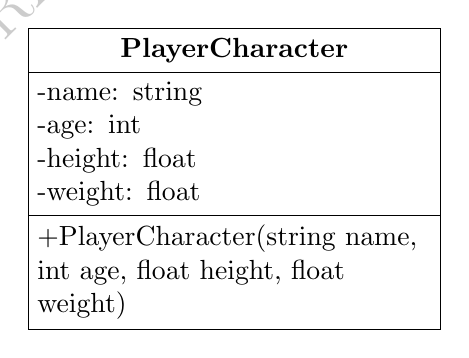
\begin{tikzpicture}
			\begin{class}{PlayerCharacter}{0,0}
				\attribute{-name: string}
				\attribute{-age: int}
				\attribute{-height: float}
				\attribute{-weight: float}
				\operation{+PlayerCharacter(string name, int age, float height, float weight)}
			\end{class}
		\end{tikzpicture}
	}

	\caption{PlayerCharacter class with various desired parameters}
	\label{fig:playercharacter-1}
\end{figure}

Using the builder pattern, we create a encapsulated structure that would contain all the parameters in figure \ref{fig:playercharacter-builder} and then default all of the struct internal variables to some default value. We then have the flexibility to fill in whichever attribute we want to change by modifying the struct's members (\texttt{struct PlayerCharacterBuilder builder; builder.age = 25;}). Optional logic could be added to the builder as well.

\begin{figure}[H]
	\centering

	\scalebox{0.75}{
		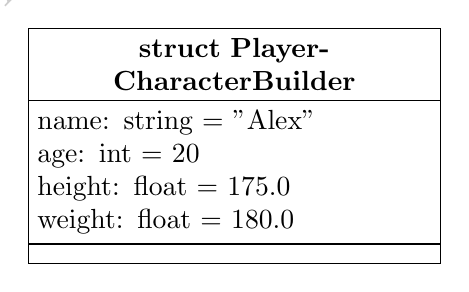
\begin{tikzpicture}
			\begin{class}{struct PlayerCharacterBuilder}{0,0}
				\attribute{name: string = "Alex"}
				\attribute{age: int = 20}
				\attribute{height: float = 175.0}
				\attribute{weight: float = 180.0}
			\end{class}
		\end{tikzpicture}
	}

	\caption{PlayerCharacterBuilder struct}
	\label{fig:playercharacter-builder}
\end{figure}

Now, the PlayerCharacter class constructor only uses a single parameter of the builder type reference (figure \ref{fig:playercharacter-2}). The constructor then reads all the values in the struct, and assign them to the corresponding member variables.

\begin{figure}[H]
	\centering

	\scalebox{0.75}{
		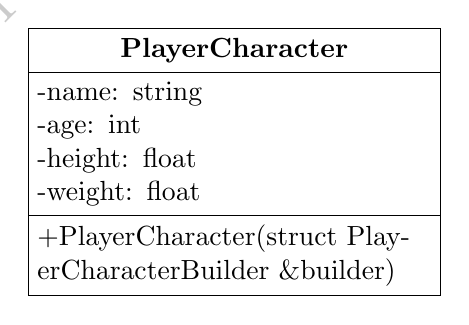
\begin{tikzpicture}
			\begin{class}{PlayerCharacter}{0,0}
				\attribute{-name: string}
				\attribute{-age: int}
				\attribute{-height: float}
				\attribute{-weight: float}
				\operation{+PlayerCharacter(struct PlayerCharacterBuilder \&builder)}
			\end{class}
		\end{tikzpicture}
	}

	\caption{PlayerCharacter class with various desired parameters}
	\label{fig:playercharacter-2}
\end{figure}

Of course, this pattern is applicable widely in game development, from in game objects that have visual variations, to online player save files, and even the build pipelines used during development to build game assets.\bs
\\
A sample code for this pattern is available in section \ref{code:builder}.

\subsection{Factories}

Factory is a quintessential creational design pattern because it governs the creation of different types of objects at a scalable level. For programming games, memory allocation and management is tricky, therefore it is helpful to not expose that kind of control to the client code.\bs
\\
The three main factories patterns we will explore is \textit{Simple Factory}, \textit{Abstract Factory}, and \textit{Factory Method}. However, because factory method pattern is very similar to abstract factory\cite{sm-factory-method} in the context we care about, we will only explore abstract factory. The general pattern in all these different factory patterns is that the keyword \texttt{new} in C++ is harmful. And that the factory should abstract away the specific steps to instantiation.\bs
\\
\textbf{Simple Factory}\\
As the name suggests, the \textit{simple factory} is as simple as a factory could get, the simple factory generates an instance for the client but does not expose any instantiation logic.\cite{simple-factory}\bs
\\
A real life analogy would be purchasing a burger: the client requests one burger, and the restaurant makes the burger and give it to the client. Without the factory design pattern, the client would need to gather all the ingredients of the burger and make it themselves, which is repetitive and unproductive.\bs
\\
(Simple factory in game development ehhhhh).\bs
\\
A sample code for this pattern is available in section \ref{code:simple-factory}.\bs
\\
\textbf{Abstract Factory}
\\
Abstract factories are useful in cases where we need to instantiate abstract objects, but we do not know the specific concrete object yet\cite{sm-abstract-factory}. This pattern is prevalent in cross-platform UI programming where the identical elements have similar characteristics, but behave slightly differently under the hood. A typical abstract factory resembles a structure depicted in figure \ref{fig:abstract-factory}.\cite{ctan-abstract-factory}\bs
\\
For instance, suppose we have a game that runs on Xbox, PlayStation, and PC, and in it we have a UI widget to enter the player name. The expected behavior would be to open the first-party on screen keyboard for the two consoles, and do nothing for PC (as keyboard is physical). In this case, to make the code more maintainable, we would not program it with two or more variants just to work with different controls.\bs
\\
A similar example is provided in the sample code in section \ref{code:abstract-factory}\cite{sm-abstract-factory-example}.\bs
\\
Of course, the abstract factory could be generalized to various mechanisms within a game from game objects to player characters.\bs
\\

\iftwocolumns
\end{multicols}
\fi

\begin{figure}[!ht]
	\centering
	\scalebox{0.55}{
		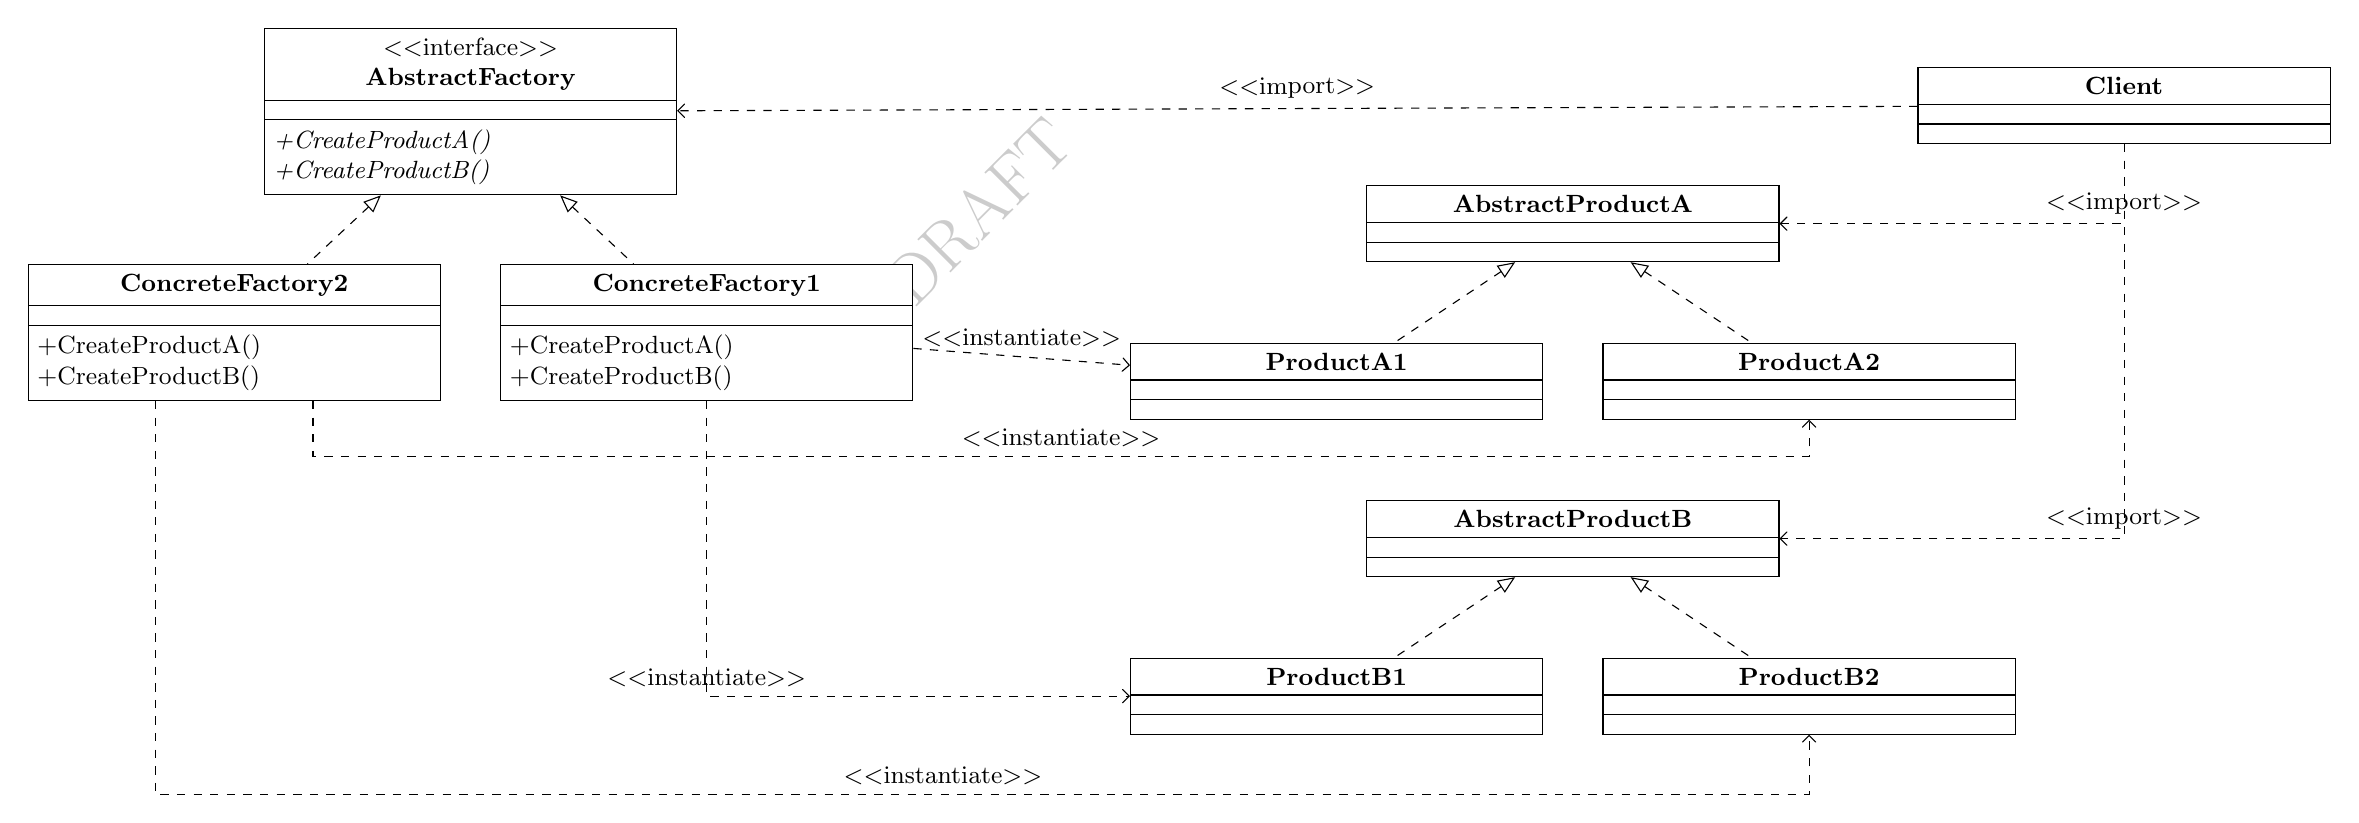
\begin{tikzpicture}
			\tikzstyle{every node}=[font=\small]
			\begin{interface}{AbstractFactory}{0, 0}
				\operation[0]{+CreateProductA()}
				\operation[0]{+CreateProductB()}
			\end{interface}
			\begin{class}{ConcreteFactory2}{-3, -3}
				\implement{AbstractFactory}
				\operation{+CreateProductA()}
				\operation{+CreateProductB()}
			\end{class}
			\begin{class}{ConcreteFactory1}{3, -3}
				\implement{AbstractFactory}
				\operation{+CreateProductA()}
				\operation{+CreateProductB()}
			\end{class}
			\begin{class}{AbstractProductA}{14, -2}
			\end{class}
			\begin{class}{ProductA1}{11 , -4}
				\implement{AbstractProductA}
			\end{class}
			\begin{class}{ProductA2}{17 , -4}
				\implement{AbstractProductA}
			\end{class}
			\draw[umlcd style dashed line, ->](ConcreteFactory1)--node[above, black]{$<<$instantiate$>>$}(ProductA1);
			\draw[umlcd style dashed line, ->](ConcreteFactory2.south)++(1, 0)--++(0, -0.7)--node[above, sloped, black]{$<<$instantiate$>>$}++(19 ,0)-|(ProductA2);

			\begin{class}{AbstractProductB}{14, -6}
			\end{class}
			\begin{class}{ProductB1}{11, -8}
				\implement{AbstractProductB}
			\end{class}
			\begin{class}{ProductB2}{17, -8}
				\implement{AbstractProductB}
			\end{class}
			\draw[umlcd style dashed line, ->](ConcreteFactory1)|- node[above, sloped, black]{$<<$instantiate$>>$}(ProductB1);
			\draw[umlcd style dashed line, ->](ConcreteFactory2.south)++(-1 ,0)--++(0, -5)--node [above, sloped, black]{$<<$instantiate$>>$}++(20, 0)-|(ProductB2);
			\begin{class}{Client}{21, -0.5}
			\end{class}
			\draw[umlcd style dashed line, ->](Client)--node[above, sloped, black]{$<<$import$>>$}(AbstractFactory);
			\draw[umlcd style dashed line, ->](Client)|-node[above, sloped, black]{$<<$import$>>$}(AbstractProductA);
			\draw[umlcd style dashed line, ->](Client)|-node[above, sloped, black]{$<<$import$>>$}(AbstractProductB);
		\end{tikzpicture}
	}
	\caption{A generic UML diagram of abstract factory pattern (source: pfg-umlcd documentation\cite{ctan-abstract-factory})}
	\label{fig:abstract-factory}
\end{figure}

\iftwocolumns
\begin{multicols}{2}
\fi

\subsection{Object Pool}

An analogy in real life would be a library of books. When a client wants to access some information, instead of writing a new book to the client to use every time, which is expensive, we check if the book already exists in the library. Then we could lend the book to the client. When the client is finished, they return the book for other clients to checkout.\bs
\\
The object pool is a creational design pattern that caches objects for re-use. An object pool can let clients check-out objects from the pool. If a requested object do not exist, the pool can create a new object; although expensive, it only occurs once. Finally, using object pool better organizes object life time of the objects in the pool. Thus we can free memory by clean up unused objects periodically (often known as \textit{garbage collection}).\bs
\\
% NOTE: textures cannot be used as example as they are more like flyweights
% An example of this used in games are cached textures: 

% TODO:
% An example of the object pool design pattern would be (StateStream from simulation threads to rendering threads).

(Objective markers that need to be displayed on the screen: they are persistent in the world, but not all of them needs to be displayed all the time. Only the ones inside players' camera frustum are rendered. But that does not mean we should destroy other markers as it would be more expensive to create them again, and could cause performance issues if the player looks around too fast (spinning). So we return the instance of the marker when they're no longer being rendered to the object pool. They will be accessible and can be rendered again when players' camera puts these markers into view.)

\subsection{Prototype}

The \textit{prototype} design pattern helps when we need to create an object that is similar to an existing one, but instantiating a new instance is relatively expensive.\bs
\\
For instance, suppose we have a procedurally generated 3D model of a rock and we want to clone this model all over the place $N$ times.\bs
\\
We could just generate $N$ rocks like how we generated the first one using the same random seed.\footnote{Procedurally generation relies on pseudo-random or noise, which are based off of a seed.} The problem is for every clone of the rock, there are computational overheads that hinders efficiency: such as re-computing the normal vectors from all the faces of the polygon, or recalculating the UV coordinates for the texture.\bs
\\
Using the prototype design pattern, we implement a clone method to the rock object that copies all its data to a new instance, thereby avoiding the re-computation overheads.

\subsection{Singleton}

The singleton pattern involves creating a single instance of a class and make sure that only one is created and used\cite{tp-singleton}. The singleton pattern provides a global accessor to the client such that it can be accessed everywhere. Thus, it is said singletons are glorified global variables.\cite{ood-singleton, sm-singleton}\bs
\\
In game development, singletons can be used for for system managers. i.e. a single manager class that overlooks and orchestrates UI system or a system to track achievements. (see section \ref{ssection:ecs} for component-entity-system architecture where a single system manages multiple objects).\bs
\\
Singletons are also useful for configuration classes and shared resource accessing classes.\cite{ood-singleton} An example in game development is levels and personalization libraries (customization) where we load them into memory during loading screen initially. After-which their instance can be accessed via a static function call.\bs
\\
Typical singleton class implementation holds a static reference to itself and a static getter that returns that reference (figure \ref{fig:singleton}). In singleton implementations, concept of \textit{Lazy implementation}, where we do not initialize and allocate the memory for the object until client actually requests it.

\begin{figure}[H]
	\centering

	\scalebox{0.75}{
		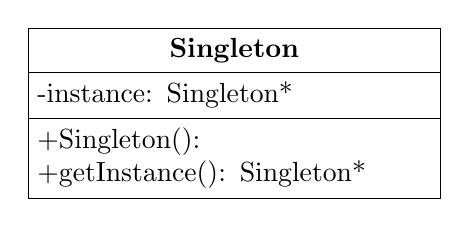
\begin{tikzpicture}
			\begin{class}{Singleton}{0,0}
				\attribute{-instance: Singleton*}
				\operation{+Singleton():}
				\operation{+getInstance(): Singleton*}
			\end{class}
		\end{tikzpicture}
	}

	\caption{Generic singleton UML class diagram}
	\label{fig:singleton}
\end{figure}

An example of Singleton implementation for an simple achievement tracker in sample code in section \ref{code:singleton}.

\section{Behavior Design Patterns}

TODO:

\subsection{Chain of Responsibility}

(InputHandlers and InputDispatchers) in Frostbite engine. A series of input handlers are chained together. Each input handler may hold reference to other input handlers.
\bs
When an input, such as mouse, keyboard, or controller action occurs. The calls traverses down the chain of input handlers until one of the input handler entities "consumes" it, which ends the chain.
\bs

Another chain of command pattern observed in the Forstbite engine editor, is handling mouse press when there are multiple \textit{hitzones}\footnote{Hitzones are interactive areas for mouse that reports data and events such as mouse position, if mouse is hover, mouse button presses and releases} overlapped (figure \ref{fig:chainofcommand-mousezones}). Any press or hovering event will be handled by the top-most hitzone entity first. If the handler does not consume the input event, the event will naturally "flow" down to the next level.
\bs

\begin{figure}[H]
	\centering
	\includegraphics[width=0.3\textwidth]{assets/chainofcommand_mousezones}
	\caption{Mouse interacting with overlapping mouse hitzones}
	\label{fig:chainofcommand-mousezones}
\end{figure}

\subsection{Command}

Decouples action request and action handlers. The callee who makes the request makes no assumptions about the class the receives the command. Effectively decoupling them.
\bs
This opens up more flexibility in mapping a requests to a handler. An example is re-mappable input handling. Instead of listening for a key press, then calling a specific function that the key press corresponds to. It invokes a command object that holds a reference to the \textit{real object} so that the handler can be called.
\bs
In between we could do more things. For instance, keep track of how many times the action has requested.
\bs
Command pattern also opens up for redo/undo operations.

\subsection{Mediator}\label{ssection:mediator}

TODO:

Mediator acts as a middle-man between communicating objects and decouples them\cite{sm-mediator}.

\begin{figure}[H]
	\centering
	\includegraphics[width=0.3\textwidth]{assets/mediator_before}
	\caption{Objects communicating without using mediator pattern}
	\label{fig:mediator-before}
\end{figure}

\begin{figure}[H]
	\centering
	\includegraphics[width=0.3\textwidth]{assets/mediator_after}
	\caption{Objects communicating using mediator pattern}
	\label{fig:mediator-after}
\end{figure}

As seen in figure \ref{fig:mediator-before}, complexity of interactions between objects become exponentially large as the software grows.
\bs
Such problem occurs often in UI: An example would be when a input signal is mapped to multiple elements. In particular, say we have a button to open up the game menu. Then at the same time there are a few systems we need to talk to during this. First, we need to tell the game to lock all inputs to the character in the world, so that when we're navigating the menu, we don't move the character around. We want to enable mouse cursor (and hide it during game play). We might want to pause the game so that enemies don't attack in the background while we have the menu open. We might want to optimize performance by turning off rendering of the world when we're in the menu, since we might not able to see it anyway.
\bs
Without using a mediator, the activated event from the button would need to invoke methods in all these different systems. This \textit{antipattern} breaks abstraction, tightly decouples all these systems together which makes it prone to error and crashes, and makes the code highly unmaintainable.
\bs
Instead, we use pattern as depicted in figure \ref{fig:mediator-after}. The button event should communicate with a middle-man that sets a state. The various systems that would be affected does not know anything about the button, or anything that interacts with the mediator. It merely gets the state stored in the mediator, and performs corresponding action.
\bs

% CHANGED: this may not be the case as shared lock is more of a 'critical system' solution
% In Frostbite, a similar mechanism is called a \textit{SharedLock}. 

\subsection{Memento}

Memento are design patterns for objects to know how to save and load (externalize) its own internal state and data.\bs
\\
Usability improvement: when used together with Command pattern, we can create undo/redo actions. Not as applicable in the game engine itself, but essential to the development tools and editors artists and scripters use to develop the game.\bs
\\

\textbf{Difference Between Command and Memento}\bs
\\

Command passes a request from the client to be handled while memento passes its own internal state. Using an analogy of how a player interacts in a game menu: a command would be the event of player clicking on the save/load buttons of their game files, and the memento would be the save file objects itself being saved/loaded.\bs
\\

\subsection{Observer}

The observer design pattern is ubiquitous to software development. Observers define a one-to-many dependency where many clients can ``subscribe'' to a state change of a particular object. The clients would be notified by the broadcast sent by the subscribed object.\bs
\\
In observer pattern, the object sending the events is the \textit{subject}, and the objects receiving are the \textit{observer}. The observer hierarchy consists of an abstract \textit{observer} base class, which has some handler (see figure \ref{fig:observer-simple}).

\begin{figure}[H]
	\centering

	\scalebox{0.75}{
		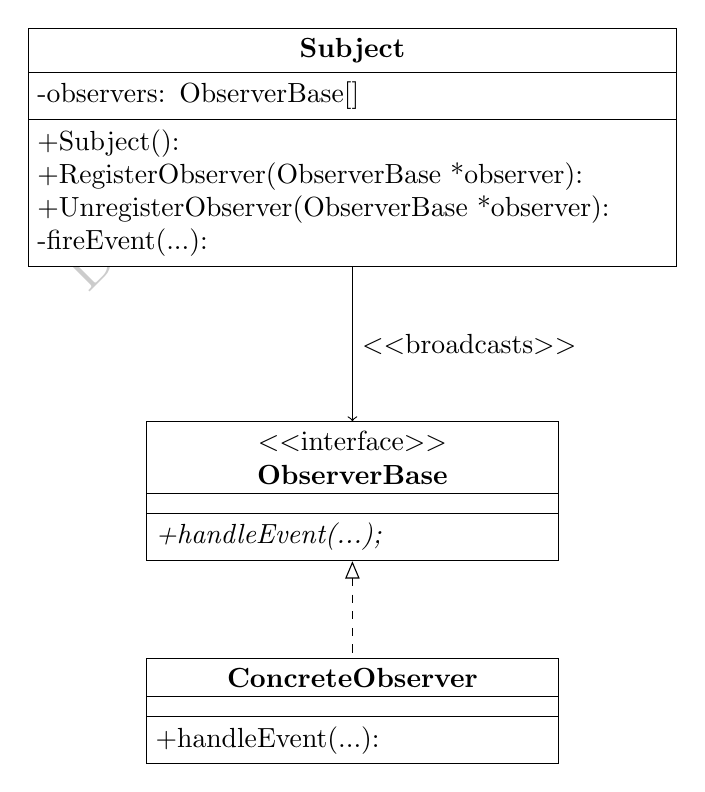
\begin{tikzpicture}
			\begin{class}[text width=8cm]{Subject}{0,0}
				\attribute{-observers: ObserverBase[]}
				\operation{+Subject():}
				\operation{+RegisterObserver(ObserverBase *observer):}
				\operation{+UnregisterObserver(ObserverBase *observer):}
				\operation{-fireEvent(...):}
			\end{class}

			\begin{interface}{ObserverBase}{0,-5}
				\operation[0]{+handleEvent(...);}
			\end{interface}

			\begin{class}{ConcreteObserver}{0, -8}
				\implement{ObserverBase}
				\operation{+handleEvent(...):}
			\end{class}

			\draw[->](Subject)--node[right, black]{$<<$broadcasts$>>$}(ObserverBase);
		\end{tikzpicture}
	}

	\caption{Simple subject-object relationship in observer design pattern}
	\label{fig:observer-simple}
\end{figure}

Without using any mediators, the subject is \textit{loosely coupled}\footnote{Loose coupling means dependency to another object via interface or abstract class. Whereas tight coupling means dependency to the concrete class directly.} to the observer types. The subject holds a collection or list of registered observers, such that when an event should be fired, the subject iterates through all the observers and deliver the event.\bs
\\
The client is responsible for managing the observers' lifetime. The client or observers are responsible for when to register or unregister to a subject. In essence, the subject makes no assumption about its observers. (Similar to the relationship in model-view-controller where the controller act as observer to the view to enable user interaction - see section \ref{ssection:ecs}).\bs
\\
In Frostbite (and extends to many game engines and software), many OOP and inter-class relationship relies on events. A player's interaction with the controller, keyboard, or mouse triggers input events to be handled by the Input Handler. For example shown in figure \ref{fig:unreal-input}, the subject are objects that outputs an event whenever certain key is pressed (red blocks). The output event \textit{Released} is hooked up to some observer. The corresponding observers are the \textit{Move Updated Component} handlers that carries out specific tasks whenever it receives the event/signal.

\begin{figure}[H]
	\centering
	\includegraphics[width=0.49\textwidth]{assets/unreal-input}
	\caption{Example of event connections in Unreal Engine which is based on the observer design pattern. \cite{gfs-input}}
	\label{fig:unreal-input}
\end{figure}

It avoids the antipattern of \textit{spaghetti code} where increase in complexity of the software leads to exponential increase in complexity and unmaintainable code. The design pattern is very useful for organization, maintainability, flexibility, and scalability of code.\bs
\\
There are several approach to the implementation. Mainly, the subject could push data to observers during the function call. Or the observers could pull data from the subject. The observers could receive a subject pointer during construction and register themselves, or a client could register the observers for them. Nonetheless, the observer pattern is flexible and fit many needs in video game programming.\bs
\\
A sample code of an observer pattern example is in section \ref{code:observer}. In this example, we created a simple system to broadcast world events to a multiplayer game.

\subsection{Visitor}
TODO:

\section{Structural Design Patterns}
TODO:

\subsection{Adapter}
TODO:

A middle layer that transforms the interface of a desired object (usually provided by libraries) to work with client.\bs
\\


\textbf{Difference Between Adapter and Mediator}\bs
\\

Different from \textit{mediators} (section \ref{ssection:mediator}), as mediator manages the communication between two classes, essentially decouples the interaction of the two. Whereas adapter simply translates.
\bs
Consider a real life analogy, where two people who speak different languages are fighting. A mediator would be a lawyer such that the two people don't talk to each other directly. An adapter would be a translator so that the two can communicate more directly. Thus, adapter is structural. And Mediator is behavioral.

\subsection{Bridge}
TODO:

\subsection{Composite}
TODO:
Useful in architectures such as component-entity-systems model which centers around the idea of ``\textit{composition over inheritance}" (section \ref{ssection:ecs}).


\subsection{Decorator}
TODO:

\subsection{Facade}
TODO:

\subsection{Flyweight}
TODO:

\subsection{Proxy}
TODO:

Smart pointers, etc.

\section{Architectural Patterns}

TODO:

\subsection{Entity-Component-System}\label{ssection:ecs}

Used in physic engines, and when there are a lot of things to handle.

% CHANGED: not used too much in UI
% In UI Systems as there are also lots of things to handle. UI widgets do not necessary need to interact with other UI widgets. So using this architecture enables performance optimizations.

Other examples include making certain objects in the physics engine adopt a characteristic: i.e. solid/has collision, soft body/hard body, and other physics-aware components.\bs
\\
It could be argued that a ``controllable'' component could exist to make certain object player-controllable (i.e player characters, car, etc.).\bs
\\
Objects could also inherit components that made them aware of inputs such as mouse. Before Frostbite uses input trees and hit-zone entities, certain UI element could attach mouse interaction components to make them respond to mouse events such as hover, enter and leaving hitzones, click, etc.\bs
\\

Update calls can be queued for all objects at once. Update states can be cached. Cached data are much faster.

\subsubsection{Composition over Inheritance}

TODO:
OOP principle that makes inheritance based on composition / behavior rather than inheritance from parent.
\bs
Consider code in section \ref{code:coi-component}, rather than defining class by their ``likeness'', we define it by its function.
\bs
Then in 

\subsection{Model-View-Controller}

TODO: Mostly used in UI development. 

% !!! [CONCLUSION]
\section{Conclusions}
TODO:

\subsection{Recommendations}
TODO:

\iftwocolumns
\end{multicols}
\fi

% !!! [BIBLIOGRAPHY]
\clearpage
\addcontentsline{toc}{section}{References}
% \bibliographystyle{apalike}
\bibliographystyle{ieeetr}
\bibliography{references}

% !!! [APPENDIX]
\clearpage
\appendix
\section{Sample Code}

\subsection{Abstract Factory}
\lstinputlisting[language=C++, firstline=79, lastline=116]{code/Factories.hpp}\label{code:abstract-factory}

\subsection{Builder}
\lstinputlisting[language=C++, firstline=5]{code/Builder.hpp}\label{code:builder}

\subsection{Composition Over Inheritance}
\subsubsection{Components}
\lstinputlisting[language=C++, lastline=26]{code/CompositionOverInheritance_1.hpp}\label{code:coi-component}
\subsubsection{Usage}
\lstinputlisting[language=C++, firstline=28]{code/CompositionOverInheritance_1.hpp}\label{code:coi-usage}

\subsection{Observer}\label{code:observer}
\subsubsection{Subject Abstract Observer Class}
The simple implementation of a observer pattern is as follows. Notice that the subject is loosely coupled to the observer. But the observer is tightly coupled to the subject.
\lstinputlisting[language=C++, lastline=72]{code/Observer.hpp}
\subsubsection{Concrete Observers}
Here are some examples of concrete observers that inherits the observer base class. They override the virtual \texttt{handleEvent} method to handle whatever they're designed to do. In this case, any instances of \textit{ZeroObservers} registered to a subject would print out ``Subject received data=0'' whenever the something calls subject's \texttt{setData()} method and passes in 0.
\lstinputlisting[language=C++, firstline=74, lastline=94]{code/Observer.hpp}
For more flexible applications, the observer also could also get a subject pointer and pull the data from the subject upon an event. Consider the following concrete observer class:
\lstinputlisting[language=C++, firstline=96, lastline=108]{code/Observer.hpp}
We invoke \texttt{getSubject()} method (to ensure we can make no changes to the subject itself) and call the getter directly.
\lstinputlisting[language=C++, firstline=111]{code/Observer.hpp}


\subsection{Simple Factory}
\lstinputlisting[language=C++, firstline=3, lastline=59]{code/Factories.hpp}\label{code:simple-factory}
\subsubsection{Not Using Factory}
Not only that we need to create the objects at first, we also need to ensure that every object is properly initialized correctly. In this case, we're using a for-loop. However, one can see that as number of things to initialize increase, and initialization gets more complex, the client would need to do much more work.
\lstinputlisting[language=C++, firstline=62, lastline=71]{code/Factories.hpp}
\subsubsection{Using Factory}
Notice that the initialization logic is hidden away at this level. So using the code is much simpler.
\lstinputlisting[language=C++, firstline=73, lastline=79]{code/Factories.hpp}

\subsection{Singleton}
\lstinputlisting[language=C++]{code/Singleton.hpp}\label{code:singleton}

% End of document
\end{document}